\section{Some difficulties}
\begin{example}
Consider the integral of $1/x^2$ on the interval $[-1,1]$.
\[\int_{-1}^1\frac{1}{x^2}\dx=\left[-\frac{1}{x}\right]_{-1}^1=\left[-\frac{1}{1}\right]-\left[-\frac{1}{-1}\right]=-2.\]

\begin{figure}[H]
\centering
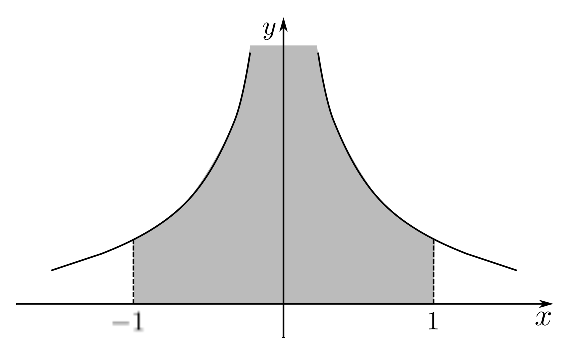
\includegraphics[scale=0.8]{img/integration-graph-over-x-squared-0}
\caption{Integrating to find the shaded area under the curve $y=\frac{1}{x^2}$ on the interval $[-1,1]$?}
\label{fig:integration-graph-over-x-squared=0}
\end{figure}

However, the area under the curve in this interval is not $-2$! What is wrong here?
\end{example}

In the above example, the integral was not the area under the curve because there was an asymptote at $x=0$. We must be sure that the function is defined
over the whole domain before we integrate.

\begin{example}
Consider the function $f(x)=x^3$. Then the integral over the interval $[-1,1]$ is
\[\int_{-1}^1x^3\dx=\left[\frac{1}{4}x^4\right]_{-1}^1=\frac{1}{4}-\frac{1}{4}=0.\]

\begin{figure}[H]
\centering
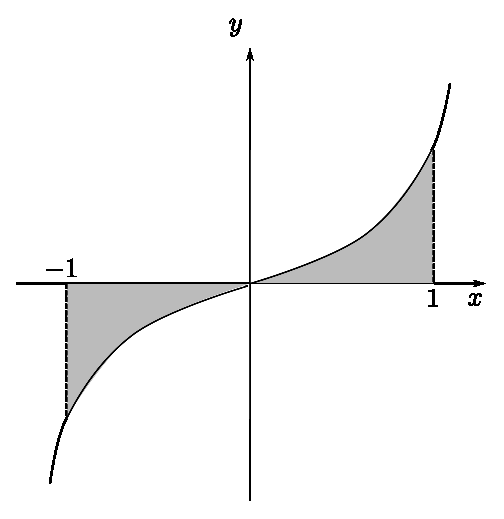
\includegraphics[scale=0.7]{img/integration-graph-x-cubed}
\caption{The area under the curve $y=x^3$ on the interval $[-1,1]$.}
\label{fig:integration-graph-x-cubed}
\end{figure}

In this case, the areas cancel out as area below the $x$-axis is negative. The shaded area is actually given by
\[\int_{0}^1x^3\dx+\left|\int_{-1}^0x^3\dx\right|=\left[\frac{1}{4}x^4\right]_0^1+\left|\left[\frac{1}{4}x^4\right]_{-1}^0\right|=\frac{1}{4}+\frac{1}{4}=\frac{1}{2}.\]
\end{example}
